% ###################################################################################################
% Chapter 3 - Physical Description
% ###################################################################################################

\chapter{Physical Description}

\begin{figure}[h]
    \centering
    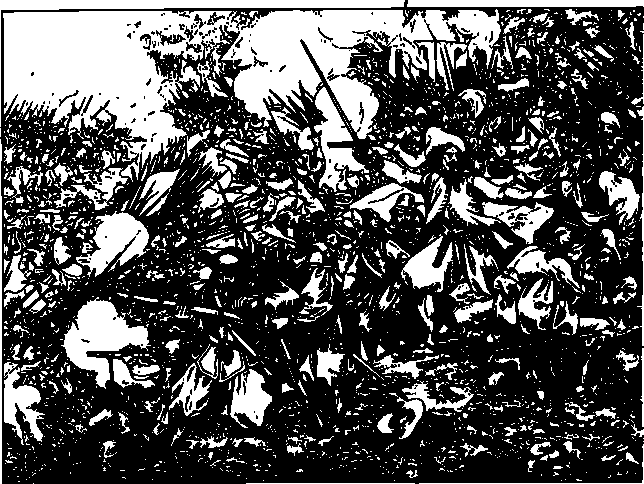
\includegraphics[width=\textwidth]{./images/physical_05.pdf}
    % \caption{Inline Example Image}
\end{figure}


This chapter delves into the intricate details that bring characters to life within the world of Eidos. As players embark on their imaginative journeys, this section serves as a guide to creating vivid and visually appealing characters. A character's physical appearance not only shapes their identity but also influences how they interact with the game's immersive setting.

Within this chapter, players will discover a wealth of options and considerations to craft the perfect physical representation of their character. From facial features and body types to hairstyles and clothing choices, each element contributes to a unique and memorable persona. Whether it's a towering warrior with a battle-scarred face, a nimble rogue with piercing eyes, or a mystical spellcaster adorned in intricate robes, the physical description chapter empowers players to manifest their characters' appearances with precision and creativity.

By providing a comprehensive exploration of physical traits, this chapter ensures that every player has the tools necessary to design characters that not only reflect their imagination but also contribute to the depth and immersion of the game world. With attention to detail and an emphasis on personal expression, Eidos encourages players to embrace their creativity and bring forth characters that will leave a lasting impression on their adventures.

\subsection{\textbf{Body}}

The human form is a canvas for storytelling, and body types play a significant role in shaping a character's physical presence. In this section, we delve into the diverse aspects of body types, starting with \textbf{Height}. Explore how height can influence perception, power dynamics, and interactions within your character's world.

\begin{itemize}
    \item Height Options:
    \begin{itemize}
        \item Tall
        \item Average
        \item Short
        \item Very Tall
        \item Very Short
    \end{itemize}
\end{itemize}

Next, we examine the concept of \textbf{Build}, exploring different body shapes and sizes and their impact on character traits and capabilities.

\begin{itemize}
    \item Build Options:
    \begin{itemize}
        \item Slender and Athletic
        \item Robust and Heavily Built
        \item Lean and Muscular
        \item Petite and Delicate
    \end{itemize}
\end{itemize}

Finally, we discuss the importance of \textbf{Proportions}, highlighting how well-balanced proportions contribute to a visually appealing and believable character.

\begin{itemize}
    \item Proportions Options:
    \begin{itemize}
        \item Well-Balanced
        \item Long Limbs
        \item Short Torso
        \item Broad Shoulders
        \item Proportionate Limbs
    \end{itemize}
\end{itemize}

Consider this expanded options for each aspect to further customize your character's height, build, and proportions. These choices will help shape your character's physical presence, traits, and visual identity within the game world.

\subsection{\textbf{Skin  - Texture}}

The skin is the outermost layer of the body, providing protection and serving as a canvas for expression. In this section, we explore the intricate aspects of skin and skintone, allowing you to create characters with diverse appearances and backgrounds.

Skin texture refers to the surface quality and appearance of the skin. It can vary from smooth and flawless to rough and weathered, adding depth and realism to your character's visual representation. Consider the following options for skin texture:

\begin{itemize}
    \item \textbf{Smooth}: Skin with a smooth and even texture, free from visible blemishes, scars, or imperfections. It appears soft, supple, and well-nourished.
    \item \textbf{Freckled}: Skin with scattered freckles across the face and sometimes other areas of the body. Freckles are small, pigmented spots that add charm and youth.
    \item \textbf{Wrinkled}: Skin with visible wrinkles and fine lines, often associated with aging or exposure to environmental factors. It appears creased or folded.
    \item \textbf{Blemished}: Skin with noticeable blemishes such as acne, pimples, or blackheads. It may appear inflamed or uneven in texture.
    \item \textbf{Dimpled}: Skin with small, natural indentations known as dimples, often seen on cheeks or chin. Dimples can add a touch of charm and playfulness.
    \item \textbf{Weathered}: Skin that shows signs of exposure to harsh elements, such as wind or sun damage. It may appear rough, dry, or aged.
    \item \textbf{Glowing}: Skin that radiates a healthy glow and appears vibrant, often associated with good health and a balanced lifestyle.
\end{itemize}

By selecting a specific skin texture, you can visually convey your character's history, lifestyle, and unique traits, enhancing their depth and storytelling potential.


\begin{figure}[h]
    \centering
    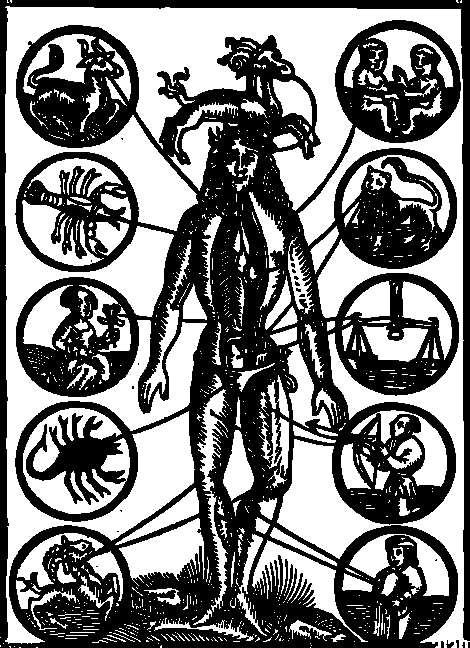
\includegraphics[width=0.5\textwidth]{./images/physical_01.pdf}
    % \caption{Inline Example Image}
\end{figure}

\subsection{\textbf{Skin  - Skintone}}

The skin is the outermost layer of the body, providing protection and serving as a canvas for expression. In this section, we explore the intricate aspects of skin and skintone, allowing you to create characters with diverse appearances and backgrounds.

\textbf{Skintone}

Skintone encompasses the coloration of the skin, which can vary across a broad spectrum. It is influenced by factors such as genetics, environment, and cultural heritage. Explore the diverse skintone options for your character:

\begin{description}
    \item[\textbf{Fair}] A light complexion with a delicate, porcelain-like appearance. Similar to fresh snow or fine china.
    \item[\textbf{Light}] A pale and subtle skintone with a soft and gentle complexion. Similar to a petal or light cream.
    \item[\textbf{Pale}] A very light skintone with minimal color and a delicate complexion. Similar to a pearl or light mist.
    \item[\textbf{Porcelain}] A smooth and pale skintone resembling fine porcelain or alabaster. Similar to fine porcelain or marble.
    \item[\textbf{Ivory}] A creamy and pale skintone with a soft, warm undertone. Similar to ivory or warm sand.
    \item[\textbf{Beige}] A warm and neutral skintone with a light tan hue. Similar to beige or light caramel.
    \item[\textbf{Natural}] A balanced and neutral skintone resembling the natural color of human skin. Similar to natural skin color or sand.
    \item[\textbf{Golden}] A warm skintone with a subtle golden hue, giving a radiant and sun-kissed appearance. Similar to golden wheat or honey.
    \item[\textbf{Peach}] A soft and warm skintone with a gentle peachy undertone. Similar to a ripe peach or apricot.
    \item[\textbf{Rosy}] A skintone with a rosy or pinkish hue, giving a healthy and youthful appearance. Similar to a rose petal or flushed cheeks.
    \item[\textbf{Warm}] A warm-toned skintone with a sun-kissed appearance and golden undertones. Similar to warm sand or sunlit bronze.
    \item[\textbf{Olive}] A skintone with a greenish or yellowish undertone, often found in individuals with Mediterranean heritage. Similar to olive skin or light khaki.
    \item[\textbf{Tawny}] A warm and tan skintone with a mix of golden and brown undertones. Similar to tawny leather or caramel.
    \item[\textbf{Caramel}] A rich and warm skintone resembling the color of caramel or toffee. Similar to caramel or warm toffee.
    \item[\textbf{Honey}] A warm and golden skintone with rich undertones, resembling the color of honey. Similar to honey or amber.
    \item[\textbf{Bronze}] A deep and warm skintone with a bronze-like appearance. Similar to a bronze sculpture or copper.
    \item[\textbf{Tan}] A medium to dark skintone with a warm and sun-kissed appearance. Similar to tanned skin or rich sand.
    \item[\textbf{Amber}] A deep and warm skintone with a reddish or amber-like hue. Similar to amber or burnt sienna.
    \item[\textbf{Sunkissed}] A warm skintone with a sun-kissed appearance, often achieved from spending time in the sun. Similar to a sun-kissed glow or bronzed skin.
    \item[\textbf{Brown}] A medium to dark skintone with brown hues and warm undertones. Similar to rich brown or dark chocolate.
    \item[\textbf{Cocoa}] A deep and rich skintone resembling the color of cocoa or dark chocolate. Similar to cocoa or dark chocolate.
    \item[\textbf{Mahogany}] A dark and warm skintone with deep reddish-brown hues. Similar to mahogany wood or chestnut.
    \item[\textbf{Chestnut}] A deep and warm skintone resembling the color of chestnuts. Similar to chestnuts or deep earth tones.
    \item[\textbf{Mocha}] A dark and rich skintone with a mix of brown and warm undertones. Similar to a mocha coffee or dark wood.
    \item[\textbf{Dark}] A deep and dark skintone with rich, dark brown hues. Similar to deep ebony or dark soil.
    \item[\textbf{Ebony}] A very dark and intense skintone, often found in individuals with African heritage. Similar to ebony wood or black velvet.
    \item[\textbf{Deep Brown}] A deep and rich brown skintone with dark undertones. Similar to deep brown or dark chocolate.
    \item[\textbf{Coffee}] A deep and rich skintone resembling the color of coffee beans. Similar to coffee beans or dark bark.
    \item[\textbf{Onyx}] A pitch-black skintone with no discernible undertones. Similar to onyx or black velvet.
\end{description}

Choosing a skintone helps define your character's ethnicity, ancestry, and cultural identity. It adds richness and authenticity to their visual portrayal, further immersing players into the world of your RPG.

\subsection{\textbf{Skin  - Complexion}}

Complexion refers to the overall appearance and condition of the skin, including factors such as brightness, clarity, and health. It can range from a radiant and flawless complexion to a more sallow or troubled one. Consider the following complexion options:

\begin{description}
    \item[\textbf{Radiant}] A complexion that appears glowing, healthy, and vibrant. The skin has a natural radiance, often associated with good health and vitality.
    \item[\textbf{Clear}] A complexion that is smooth, even, and free from blemishes or imperfections. The skin appears flawless and has a naturally clear and bright tone.
    \item[\textbf{Ruddy}] A complexion that has a reddish or rosy undertone, often associated with a healthy flush. The skin appears lively, with a natural rosy hue.
    \item[\textbf{Sallow}] A complexion that has a yellowish or pale undertone, often associated with fatigue or illness. The skin appears dull or lacking in vitality.
    \item[\textbf{Acne-Prone}] A complexion that is prone to acne breakouts or blemishes. The skin may have visible pimples, redness, or inflammation due to acne or oily skin.
\end{description}

By selecting a specific complexion, you can add another layer of detail to your character, highlighting their physical well-being, lifestyle, or even their struggles.

Create characters with unique skin textures, skintones, and complexions to represent a wide range of backgrounds, ethnicities, and experiences. The choices you make in this aspect of character creation contribute to their visual identity and help shape their story within the game world.

\subsection{\textbf{Eyes - Colors}}

The face is a canvas that reveals the uniqueness and character of a person. In this section, we delve into the intricacies of facial features, exploring the mesmerizing world of eyes, the windows to the soul. Discover how the shape, color, and expression of the eyes can add depth and personality to your character.

\begin{description}
    \item[Brown] A warm, earthy color resembling the rich tones of coffee beans, chestnuts, or fertile soil. It can range from light caramel to deep chocolate, mirroring the shades found in the bark of trees or the feathers of certain birds.
    \item[Blue] Reminiscent of a clear sky or the shimmering surface of a calm lake, blue eyes vary from a pale, icy blue to a vibrant sapphire or deep indigo. They can evoke images of serene waters, delicate flowers like forget-me-nots, or the wings of certain butterflies.
    \item[Green] Reflecting the lushness of the natural world, green eyes can range from a vibrant emerald to a soft, mossy green. They resemble the color of fresh grass, leaves in a dense forest, or the captivating iridescence of certain gemstones like jade or malachite.
    \item[Hazel] A captivating mix of colors, hazel eyes showcase various hues such as warm browns, soft greens, and hints of gold. They can resemble the vibrant shades seen in autumn leaves, a cup of creamy hazelnut coffee, or the dappled patterns on the wings of butterflies or birds.
    \item[Gray] Exhibiting a cool and subtle tone, gray eyes can resemble the color of storm clouds, morning mist, or the feathers of certain birds like pigeons or doves. They can also have a silvery sheen, reminiscent of moonlit nights or the reflective surface of a calm lake.
    \item[Amber] Radiating a warm, golden color, amber eyes resemble the glowing embers of a cozy fire or the rich hues of autumn leaves basking in sunlight. They can bring to mind the warm glow of a candle or the golden strands of honey dripping from a spoon.
    \item[Violet] A mesmerizing purple color reminiscent of delicate lavender fields, royal amethyst gemstones, or the petals of enchanting flowers like violets or orchids. Violet eyes can evoke a sense of mystery, magic, and ethereal beauty.
    \item[Black] Deep and intense, black eyes are as dark as a moonless night. They can resemble the glossy feathers of certain birds, the obsidian surface of volcanic rock, or the captivating darkness of a starless sky.
    \item[Red] Unusual and captivating, red eyes possess a vibrant crimson hue that can resemble the fiery glow of molten lava, the intensity of a blazing fire, or the striking color of a red rose in full bloom. They convey a sense of passion, intensity, or otherworldly allure.
    \item[Violet-Blue] A captivating fusion of violet and blue, violet-blue eyes exhibit a mesmerizing shade reminiscent of a twilight sky. They can resemble the hues seen during a breathtaking sunset, the delicate petals of blue violets, or the radiant colors found in certain gemstones like tanzanite.
    \item[Gray-Blue] A subtle blend of gray and blue, gray-blue eyes have a cool and calming appearance. They can bring to mind the colors of a misty morning sky, the soft reflection on a calm lake, or the delicate patterns on seashells washed ashore.
    \item[Green-Hazel] Combining the beauty of green and hazel, green-hazel eyes showcase a captivating mix of warm greens, golden browns, and hints of amber. They can resemble the lush tones found in a sun-dappled forest, the intricate patterns on a butterfly's wings, or the vibrant colors of certain gemstones like peridot.
    \item[Gold] Resembling the precious metal it is named after, gold eyes possess a radiant and luminous hue. They can evoke images of the golden rays of the sun, the shimmering surface of a calm lake reflecting sunlight, or the warm glow of a candle flame.
    \item[Silver] Exhibiting a cool and striking appearance, silver eyes have a silvery-gray or bluish-gray hue reminiscent of moonlit nights, shimmering frost, or the reflective surface of a calm lake. They convey a sense of grace, wisdom, and a touch of enchantment.
    \item[Turquoise] A vibrant and captivating color reminiscent of the gemstone it is named after, turquoise eyes showcase a mix of blue and green tones. They can resemble the hues found in tropical waters, the iridescent feathers of certain birds like peacocks, or the mesmerizing colors of a coral reef.
    \item[Topaz] Resembling the warm, golden-brown tones of the gemstone, topaz eyes radiate a captivating charm. They can evoke images of the sun's golden rays, the rich colors of a harvest field, or the luminous glow of a bonfire on a cool evening.
    \item[Sapphire] Like the deep blue gemstone it is named after, sapphire eyes possess a rich and captivating blue hue. They evoke a sense of depth, allure, and a touch of sophistication, akin to the depths of the ocean or the clarity of a pristine waterfall.
    \item[Emerald] Radiating a lush and vibrant green color, emerald eyes capture attention and convey a sense of vitality, growth, and natural elegance. They can resemble the verdant shades of emerald gemstones, the vibrant foliage of a tropical rainforest, or the glimmering surface of a tranquil pond.
    \item[Amethyst] A captivating purple color reminiscent of the gemstone it shares its name with, amethyst eyes possess a rich, violet-purple hue. They exude an air of mystery, enchantment, and a touch of royalty. They can bring to mind the deep hues of amethyst crystals or the delicate petals of lavender flowers.
\end{description}

\subsection{\textbf{Eyes - Shapes}}

\begin{description}
    \item[Round] The most common shape, often associated with innocence and openness.
    \item[Almond] A graceful and elongated shape, often symbolizing elegance and sensuality.
    \item[Hooded] Characterized by a heavy upper lid, conveying a sense of mystery and secrecy.
    \item[Deep-Set] Set deeply into the sockets, creating an intense and soulful appearance.
    \item[Wide-Set] Positioned farther apart, suggesting a more open and friendly expression.
    \item[Upturned] Featuring an upward tilt at the outer corners, expressing a playful and mischievous nature.
    \item[Downturned] Sloping downwards at the outer corners, reflecting a hint of sadness or weariness.
    \item[Monolid] Smooth, without a visible crease, common in East Asian and Southeast Asian cultures.
    \item[Protruding] Extending outward from the face, often associated with an intense and observant gaze.
\end{description}

\subsection{\textbf{Eyes - Sizes}}

When considering eye sizes, it's important to note that there is a wide range of natural variation. The size of the eyes can contribute to the overall appearance and expression of a character. Here are some common descriptors:

\begin{itemize}
    \item \textbf{Large:} Expressive, captivating, and often associated with innocence or a childlike quality.
    \item \textbf{Small:} Intense, focused, and can convey a sense of mystery or intensity.
    \item \textbf{Average:} Balanced and versatile, suitable for a wide range of character types.
    \item \textbf{Uneven:} Different-sized eyes can add a unique and intriguing element to a character's appearance, highlighting their individuality.
\end{itemize}

\subsection{\textbf{Eyes - Eyelashes}}

\begin{itemize}
    \item \textbf{Long:} Dramatic and attention-grabbing lashes that enhance the character's gaze.
    \item \textbf{Thick:} Dense and voluminous lashes that give a fuller appearance to the eyes.
    \item \textbf{Curled:} Lashes that are naturally curled or enhanced with curlers, creating an expressive and alluring look.
    \item \textbf{Sparse:} Thin or sparsely distributed lashes that can convey subtlety, vulnerability, or a delicate beauty.
    \item \textbf{Natural:} Unadorned lashes that appear as they are, emphasizing a natural and effortless beauty.
\end{itemize}

\begin{figure}[h]
    \centering
    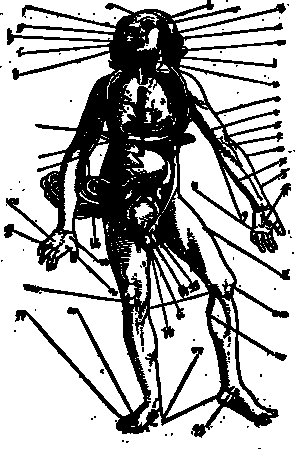
\includegraphics[width=0.5\textwidth]{./images/physical_04.pdf}
    % \caption{Inline Example Image}
\end{figure}

\subsection{\textbf{Eyes - Eyebrows}}

\begin{itemize}
    \item \textbf{Arched:} Graceful curves that add elegance and intensity to the eyes.
    \item \textbf{Straight:} Horizontal brows that give a calm and balanced appearance.
    \item \textbf{Thin:} Delicate and slender brows that can evoke a sense of refinement or fragility.
    \item \textbf{Thick:} Full and prominent brows that convey strength and boldness.
    \item \textbf{Angular:} Sharply defined angles that create a striking and expressive look.
\end{itemize}

\subsection{\textbf{Nose - Shapes}}

Among the distinguishing features of the face, the nose holds a significant role in defining a character's appearance. In this section, we explore the various shapes, sizes, and nuances of noses, uncovering how this subtle yet prominent feature can contribute to the overall characterization of your creation.

When creating a character, the choice of nose shape holds great importance in defining their appearance and personality. The selected nose shape adds depth and nuance to the character's visual portrayal, contributing to their overall characterization. Whether it's a straight nose, conveying a sense of balance and refinement, or a Roman nose, symbolizing strength and authority, each shape helps players envision their character's traits and role in the game world. By choosing a specific nose shape, players can bring their characters to life, aligning their physical features with their desired persona and enhancing the immersive experience of character creation.

\begin{itemize}
    \item \textbf{Straight:} A nose with a straight bridge, often associated with elegance and symmetry. It portrays a sense of balance and can contribute to a refined and classic appearance.
    \item \textbf{Roman:} Also known as an aquiline nose, it has a prominent bridge with a slight downward curve. This shape can evoke a sense of strength, authority, and nobility.
    \item \textbf{Button:} Characterized by a small, rounded tip, the button nose exudes a charming and youthful appeal. It is often associated with cuteness, innocence, and a playful demeanor.
    \item \textbf{Upturned:} With a slightly upturned tip, this nose shape creates an appearance of perkiness and whimsy. It can add a touch of quirkiness or mischievousness to a character's countenance.
    \item \textbf{Snub:} The snub nose features a short and slightly upturned tip, often coupled with a slightly concave bridge. It can convey a sense of charm, impishness, or a hint of rebelliousness.
    \item \textbf{Greek:} Resembling the sculptures of ancient Greek gods, this nose shape has a straight bridge and a narrow, well-defined tip. It exudes an aura of elegance, grace, and timeless beauty.
    \item \textbf{Hawk:} Similar to the beak of a hawk, this nose shape has a prominent, curved bridge with a sharp downward angle. It can portray an assertive, confident, and strong-willed character.
    \item \textbf{Snorkel:} Unconventional and unique, the snorkel nose has an extended and protruding shape resembling a snorkel tube. It adds a distinctive and eccentric touch to a character's appearance.
    \item \textbf{Crooked:} Characterized by a noticeable deviation from a straight line, the crooked nose exhibits an asymmetrical shape. It can suggest a rugged, unconventional, or mysterious persona.
    \item \textbf{Flat:} Featuring a minimal bridge height, the flat nose has a broad and low profile. It is often associated with certain ethnicities and can convey a sense of heritage, cultural identity, or natural beauty.
\end{itemize}

\subsection{\textbf{Nose - Sizes}}

In character creation, the size of the nose plays a significant role in shaping the character's visual identity. The chosen nose size can convey various attributes and characteristics, influencing how the character is perceived by others. A small nose may suggest delicacy, grace, or subtlety, while a large nose can imply strength, resilience, or even dominance. Players have the opportunity to carefully consider the impact of their character's nose size, ensuring it aligns with their envisioned persona and adds depth to their character's visual representation.

\begin{itemize}
    \item \textbf{Small:} A small nose is delicate and petite in proportion to the face. It can convey a sense of gracefulness, refinement, or youthful innocence.
    \item \textbf{Medium:} A medium-sized nose is considered average in proportion to the face. It is versatile and can complement various facial features, providing a balanced and harmonious appearance.
    \item \textbf{Large:} A large nose is more prominent and commanding, drawing attention to the center of the face. It can suggest strength, character, and individuality.
    \item \textbf{Long:} A long nose extends vertically, with a noticeable length between the bridge and the tip. It can add an elegant and regal touch to a character's countenance.
    \item \textbf{Short:} A short nose is characterized by its reduced length, creating a compact and concise appearance. It can contribute to a youthful or cute expression.
\end{itemize}

\subsection{\textbf{Nose - Nuances}}

The unique features of a character's nose are important elements in the character creation process. From the presence of a bridge bump or a nasal ridge to the absence of any pronounced features, these details contribute to the character's overall appearance and storytelling potential. A bridge bump can imply ruggedness or a history of battles fought, while a nasal ridge might signify a strong and resolute character. Conversely, a lack of notable features can add an air of simplicity or mystery to the character. By incorporating these nose features into the character creation process, players can further customize their characters, adding depth and uniqueness to their narrative experiences.

\begin{itemize}
    \item \textbf{Rounded:} A rounded nose has soft, curved contours, giving a gentle and approachable impression. It can convey warmth, friendliness, and a nurturing nature.
    \item \textbf{Angular:} An angular nose has sharp and well-defined features, with distinct lines and angles. It can suggest strength, determination, and a more assertive personality.
    \item \textbf{Tapered:} A tapered nose gradually narrows towards the tip, creating a sleek and refined appearance. It can add a touch of elegance and sophistication to a character's face.
    \item \textbf{Broad:} A broad nose has a wider shape, often with a more substantial base. It can convey a sense of strength, vitality, and resilience.
    \item \textbf{Pointed:} A pointed nose features a defined and sharp tip, adding a distinctive and slightly exotic element to a character's facial structure. It can evoke a sense of intrigue and allure.
    \item \textbf{Upward-Turned:} With an upward turn at the tip, this nose nuance creates a cheerful and optimistic expression. It can contribute to a character's cheerful, lively, or mischievous demeanor.
    \item \textbf{Downturned:} A downturned nose has a slight droop at the tip, creating a subtle melancholic or pensive look. It can suggest a reflective, introspective, or more serious disposition.
    \item \textbf{Upward-Bridge:} This nuance describes a nose with an elevated bridge, adding a distinctive feature to a character's facial structure. It can create a regal, refined, or statuesque appearance.
    \item \textbf{Flat-Bridge:} A flat bridge indicates a nose with a minimal or flattened nasal bridge. It can be associated with certain ethnicities or convey a unique and unconventional character.
\end{itemize}

\subsection{\textbf{Mouth}}

The mouth is a gateway to expression, communication, and emotion. It is a focal point of the face that can greatly influence the portrayal of a character. In this section, we delve into the captivating aspects of the mouth, including the shape of the lips, the positioning of the teeth, and the overall structure. Discover how the mouth can convey a wide range of feelings, add realism to your character, and further enhance the immersive experience of character creation.

\begin{figure}[h]
    \centering
    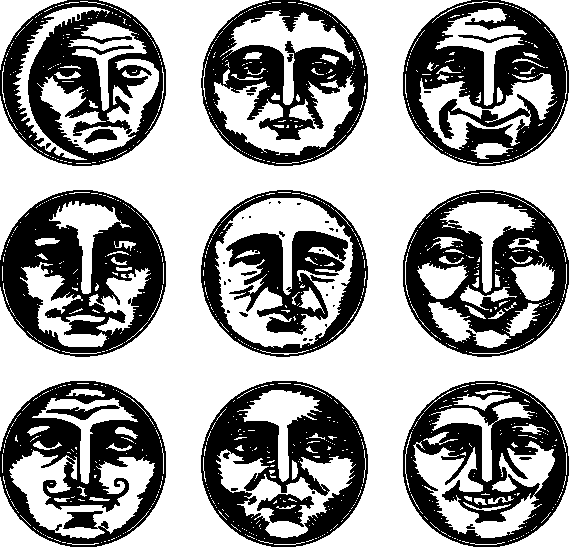
\includegraphics[width=0.5\textwidth]{./images/physical_02.pdf}
    % \caption{Inline Example Image}
\end{figure}

\subsection{\textbf{Lip Shapes}}

The shape of the lips is a defining characteristic that can communicate various emotions and traits. From full and plump lips to thin and delicate ones, each shape adds depth and nuance to a character's appearance. Full lips can signify sensuality, confidence, or a bold personality, while thin lips may suggest subtlety, reservation, or a more reserved nature. By selecting a specific lip shape, players can visually express their character's disposition and evoke certain emotions within the game world, enhancing the interactive storytelling experience.

\subsection{\textbf{Teeth Positioning}}

The positioning of teeth can contribute to the overall aesthetic of a character's mouth and provide insights into their background or lifestyle. Whether it's perfectly aligned teeth, slightly crooked teeth, or even missing teeth, each positioning tells a story. Straight teeth may denote good oral hygiene and care, while crooked teeth might suggest a rugged or unconventional nature. Missing teeth can be indicative of a character's past battles or a harsh life. By considering the positioning of teeth, players can further develop their character's backstory and create a visually striking representation.

\begin{itemize}
    \item \textbf{Straight:} Perfectly aligned teeth, indicating good oral hygiene and care.
    \item \textbf{Slightly Crooked:} Teeth with a slight misalignment, adding character and charm.
    \item \textbf{Overbite:} Upper front teeth overlapping the lower teeth, creating a unique and distinctive look.
    \item \textbf{Underbite:} Lower front teeth overlapping the upper teeth, conveying a strong or aggressive appearance.
    \item \textbf{Missing Teeth:} Gaps or missing teeth that imply a rugged past or difficult life experiences.
    \item \textbf{Fanged:} Prominent canine teeth that evoke a primal or vampiric aesthetic.
\end{itemize}

\subsection{\textbf{Mouth Structure}}

The overall structure of the mouth encompasses various elements, such as the width, depth, and curvature of the lips, as well as the shape and prominence of the jawline. These aspects significantly impact a character's visual identity and can evoke different impressions. A wide and expressive mouth can convey openness, vitality, or even a mischievous nature. A narrower mouth may imply a more reserved demeanor or a hint of mystery. The prominence of the jawline can suggest strength, determination, or elegance. By carefully considering the structure of the mouth, players can fine-tune their character's appearance and enrich their narrative journey within the game.

\begin{itemize}
    \item \textbf{Wide and Expressive:} A mouth with a generous width, capable of displaying a range of emotions with ease.
    \item \textbf{Narrow and Refined:} A more compact mouth with a slender width, suggesting a refined and reserved nature.
    \item \textbf{Strong Jawline:} A pronounced and chiseled jawline that exudes strength, determination, and resilience.
    \item \textbf{Soft and Rounded:} A gentle curve and rounded features, conveying a softer and more approachable demeanor.
    \item \textbf{Angular and Sharp:} Well-defined angles and sharp edges, projecting a more striking and intense presence.
    \item \textbf{Prominent Chin:} A prominent or elongated chin that adds a touch of distinction and character to the mouth area.
\end{itemize}

\subsection{\textbf{Chin Shape}}

The chin, with its diverse forms and contours, plays a crucial role in defining a character's facial structure. It can greatly impact the overall visual identity and contribute to the characterization of your creation. In this section, we explore the significance of chin shape, size, and prominence, and how they can add depth and realism to your character's appearance.

The shape of the chin can vary greatly, from rounded and soft to square and angular, each with its own unique characteristics. Chin shape not only affects the visual balance of the face but also conveys specific traits and qualities. A rounded chin often suggests a gentle and approachable nature, while a square chin can imply strength and determination. By selecting a specific chin shape, players can enhance their character's personality and bring their vision to life within the game world.

\begin{itemize}
    \item \textbf{Rounded:} A soft, curved chin that exudes warmth and approachability.
    \item \textbf{Square:} An angular and well-defined chin that signifies strength and resilience.
    \item \textbf{Pointed:} A chin that tapers to a subtle point, adding a touch of elegance and refinement.
    \item \textbf{Cleft:} A distinctive vertical indentation or "cleft" in the chin, creating a unique and memorable feature.
    \item \textbf{Protruding:} A chin that juts forward slightly, conveying assertiveness and confidence.
    \item \textbf{Receding:} A chin that appears slightly indented or set back, suggesting a more reserved or introverted nature.
\end{itemize}

\subsection{\textbf{Chin Size and Prominence}}

The size and prominence of the chin can significantly influence the overall facial structure and appearance. Whether it's a small and subtle chin or a prominent and commanding one, each size brings its own character and aesthetic. A small chin may suggest delicacy or a more reserved demeanor, while a prominent chin can convey strength and authority. By carefully considering the size and prominence of the chin, players can further refine their character's visual identity and create a captivating representation.

\begin{itemize}
    \item \textbf{Small:} A subtle and petite chin that adds a touch of delicacy and vulnerability to the face.
    \item \textbf{Moderate:} A balanced and proportionate chin size that suits a wide range of facial features and expressions.
    \item \textbf{Prominent:} A strong and prominent chin that commands attention and conveys power and authority.
    \item \textbf{Double Chin:} A chin characterized by an extra layer of fat or skin, creating a distinct feature with a unique charm.
    \item \textbf{Weak:} A chin with less prominent definition, suggesting a softer or more gentle disposition.
    \item \textbf{Strong:} A robust and well-defined chin that reflects determination, resilience, and assertiveness.
\end{itemize}

\begin{figure}[h]
    \centering
    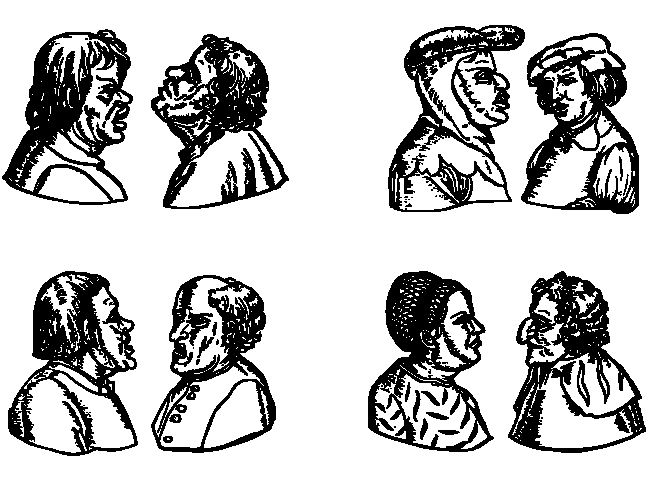
\includegraphics[width=0.8\textwidth]{./images/physical_03.pdf}
    % \caption{Inline Example Image}
\end{figure}

\subsection{\textbf{Hair Length}}

Hairstyles are a striking and versatile way to define a character's appearance, personality, and cultural background. In this section, we embark on a journey through the realm of hairstyles, beginning with considerations of **Length**. Discover how different hair lengths can evoke specific impressions and convey character traits. We then explore the **Texture** of hair, from sleek and straight to curly and voluminous, and the impact it has on character portrayal. Finally, we delve into the realm of **Style**, exploring various cuts, braids, updos, and more, and their potential symbolism and narrative significance.

A character's hairstyle can speak volumes about their personality, culture, and time period. In this section, we explore the different lengths of hairstyles, from short and cropped to long and flowing. Discover how the choice of hairstyle can shape your character's visual identity.

\begin{itemize}
    \item \textbf{Short and Cropped:} A short and neat hairstyle, often associated with practicality and efficiency.
    \item \textbf{Pixie Cut:} A short hairstyle that exudes confidence and a hint of playfulness.
    \item \textbf{Bob:} A versatile and classic hairstyle that can be worn at different lengths.
    \item \textbf{Medium-Length:} A medium-length hairstyle that offers a balance between practicality and versatility.
    \item \textbf{Shoulder-Length:} A hairstyle that falls just below the shoulders, providing a feminine and graceful look.
    \item \textbf{Long and Flowing:} Luxurious and captivating, this hairstyle is associated with elegance and femininity.
    \item \textbf{Waist-Length:} An impressive hairstyle that showcases length and dedication to hair care.
    \item \textbf{Bra Strap Length:} A popular choice that allows for various styling options and is versatile for different occasions.
    \item \textbf{Hip-Length:} A dramatic and attention-grabbing hairstyle that demands admiration.
    \item \textbf{Floor-Length:} An extraordinary hairstyle that signifies uniqueness and extravagance.
\end{itemize}

\subsection{\textbf{Hair Texture}}

The texture of a character's hair adds depth and realism to their appearance. In this section, we delve into the variety of hair textures, from straight and smooth to curly and voluminous. Learn how to incorporate the texture of hair into your character's visual profile.

\begin{itemize}
    \item \textbf{Straight and Smooth:} Sleek and glossy, this hair texture is associated with sophistication and elegance.
    \item \textbf{Wavy and Textured:} A natural and effortless hair texture that adds movement and personality to the character's look.
    \item \textbf{Curly and Voluminous:} Bouncy and full of life, this hair texture conveys a sense of energy and playfulness.
    \item \textbf{Coiled and Springy:} Spiraled and defined, this hair texture is often associated with strength and resilience.
    \item \textbf{Kinky and Natural:} Embracing the natural texture of hair, this style exudes confidence and cultural pride.
    \item \textbf{Frizzy and Untamed:} An unruly and wild texture that adds an element of rebellion and non-conformity to the character's appearance.
    \item \textbf{Silky and Fine:} Soft and delicate, this hair texture evokes a sense of grace and refinement.
    \item \textbf{Thick and Luscious:} Abundant and voluminous, this hair texture represents vitality and abundance.
    \item \textbf{Tightly Coiled and Dense:} Dense and tightly coiled, this hair texture showcases a unique and distinctive beauty.
    \item \textbf{Wiry and Textured:} A textured and coarse hair type that brings a rugged and adventurous element to the character's look.
\end{itemize}

\subsection{\textbf{Hair Color}}

Hair color is another essential aspect of a character's appearance. It can range from natural shades to bold and vibrant hues. Choose the hair color that best suits your character's personality and style.

\begin{itemize}
    \item \textbf{Blonde:} A light hair color reminiscent of sunshine and youthfulness.
    \item \textbf{Brunette:} A dark hair color that is often associated with sophistication and elegance.
    \item \textbf{Red:} A fiery and vibrant hair color that adds a bold and passionate touch to the character's appearance.
    \item \textbf{Black:} A dark and mysterious hair color that exudes a sense of intensity and depth.
    \item \textbf{Brown:} A versatile and natural hair color that ranges from light to dark shades, offering a warm and inviting look.
    \item \textbf{Auburn:} A reddish-brown hair color that combines elements of both red and brown, creating a rich and captivating hue.
    \item \textbf{Silver/Grey:} A unique and striking hair color that can symbolize wisdom, maturity, or even futuristic elements.
    \item \textbf{Platinum Blonde:} An icy and pale shade of blonde that emanates an ethereal and otherworldly aura.
    \item \textbf{Blue:} A bold and unconventional hair color that represents uniqueness and creativity.
    \item \textbf{Pink:} A vibrant and playful hair color that adds a whimsical and youthful charm to the character's appearance.
    \item \textbf{Purple:} A mystical and enchanting hair color that embodies creativity and a touch of mystery.
    \item \textbf{Green:} A fresh and nature-inspired hair color that symbolizes growth and harmony.
    \item \textbf{Burgundy:} A deep and rich shade of red that exudes elegance and a sense of luxury.
    \item \textbf{Platinum:} A cool-toned blonde hair color with a silvery sheen, creating a modern and sleek look.
    \item \textbf{Chocolate Brown:} A warm and rich shade of brown that evokes a sense of comfort and familiarity.
    \item \textbf{Ash Blonde:} A cool and ashy shade of blonde that adds a contemporary and sophisticated vibe to the character's appearance.
    \item \textbf{Ginger:} A vibrant and warm hair color with reddish undertones, often associated with spunk and individuality.
    \item \textbf{Salt and Pepper:} A mixture of grey and dark hair, representing maturity and a distinguished presence.
    \item \textbf{Mahogany:} A deep and reddish-brown hair color that brings warmth and depth to the character's overall look.
    \item \textbf{Copper:} A fiery and vibrant shade of orange-red hair color that radiates energy and passion.
\end{itemize}

\subsection{\textbf{Facial Hair}}

From beards to mustaches, facial hair can significantly alter the appearance and personality of a character. It adds another layer of depth and individuality to your creation, allowing you to further customize and define their unique style. In this section, we explore the different styles, lengths, and grooming techniques for facial hair, enabling you to bring your character to life within the game world. Beards come in various styles, each with its own distinct aesthetic and connotations. They can range from a full, bushy beard to a neatly trimmed goatee. By selecting a specific beard style, players can convey their character's personality, culture, or even occupation. Whether it's a rugged and untamed look or a meticulously groomed beard, the chosen style adds character and visual interest to the overall design.

\begin{itemize}
    \item \textbf{Full Beard:} A dense and voluminous beard that covers the entire lower face, exuding a sense of masculinity and maturity.
    \item \textbf{Goatee:} A facial hair style that focuses on the chin, featuring a small beard or tuft of hair, often accompanied by a clean-shaven upper lip. It can project a sleek and stylish image.
    \item \textbf{Stubble:} A short, intentionally unshaven look that gives the appearance of light facial hair growth. It can evoke a sense of ruggedness or nonchalant charm.
    \item \textbf{Soul Patch:} A small, trimmed patch of hair just below the lower lip, providing a subtle and distinctive facial hair accent.
    \item \textbf{Sideburns:} Strips of facial hair that extend from the hairline down the sides of the face, varying in length and thickness. Sideburns can add a touch of vintage or rebellious flair.
    \item \textbf{Mutton Chops:} Long, thick sideburns that extend downward to the jawline, creating a distinctive and bold appearance.
    \item \textbf{Handlebar Mustache:} A mustache with long, upwardly curved ends, often styled with wax for added flair. It conveys a sense of sophistication and old-world charm.
\end{itemize}

\subsection{\textbf{Beard Lengths}}

The length of facial hair plays a significant role in defining the character's appearance and can communicate different messages. From a clean-shaven look to a majestic wizard-like beard, the chosen length contributes to the character's personality and story. Selecting a specific beard length allows players to create a visual representation that aligns with their character's journey and role within the game world.

\begin{itemize}
    \item \textbf{Clean-Shaven}: A smooth and completely hairless face, suggesting youthfulness, freshness, or a meticulous grooming routine.
    \item \textbf{Short}: A short beard length that provides a hint of facial hair growth, adding a touch of maturity or ruggedness to the character's appearance.
    \item \textbf{Medium}: A moderate beard length that falls between short and long, striking a balance between refinement and masculinity.
    \item \textbf{Long}: A lengthy beard that exudes wisdom, power, or an untamed wildness. It can convey a character's journey, age, or connection to nature.
    \item \textbf{Epic}: An extraordinarily long and majestic beard that symbolizes reverence, ancient wisdom, or even divine status.
\end{itemize}

\subsection{\textbf{Hair and Beard Grooming}}

Haircare goes beyond styling; it involves maintaining the health and vitality of one's hair. In this section, we delve into the world of hair care, discussing different hair types, care routines, and products. Learn how to keep your character's locks lustrous and well-maintained. Facial hair requires maintenance and grooming to maintain its desired style and appearance. Different grooming techniques can enhance the overall look of the character's facial hair, making it appear well-kept and intentional. Players can choose from various grooming techniques to add authenticity and attention to detail to their character's facial hair.

\begin{itemize}
    \item \textbf{Stylized Stubble}: A precisely maintained and shaped stubble, giving a deliberate and fashionable appearance.
    \item \textbf{Elaborate Beard Art}: Intricate designs or patterns crafted within the facial hair, showcasing creativity and attention to detail.
    \item \textbf{Polished Mustache}: A well-groomed mustache that is perfectly shaped, trimmed, and waxed to achieve a sophisticated and distinguished look.
    \item \textbf{Beard Oil Care}: Regular application of beard oil to keep the facial hair nourished, soft, and healthy, resulting in a well-groomed and luxurious appearance.
    \item \textbf{Retro Mutton Chops}: Mutton chops styled with a vintage flair, incorporating grooming techniques from a bygone era, adding a touch of nostalgia to the character's appearance.
    \item \textbf{Wild and Untamed}: Unkempt and free-flowing facial hair that conveys a sense of rebellion, unpredictability, or a rugged and independent spirit.
    \item \textbf{Razor-Sharp Lines}: Precisely defined and sharp lines created along the edges of the beard or mustache, highlighting clean-cut grooming and meticulous attention to detail.
\end{itemize}

\subsection{\textbf{Scars}}

Scars tell stories etched onto a character's body, revealing their past experiences. Discover the significance of scars in different areas of the body and how they can shape a character's visual identity. We then delve into the world of tattoo designs, discussing various motifs, styles, and cultural inspirations. Lastly, we explore the symbolism behind scars and tattoos, unraveling the deeper meanings and connections they hold within a character's narrative.

Scars come in various types, each with its own characteristics and implications. Understanding different scar types can help in crafting a character's backstory and visual representation. In this section, we explore common scar types and their meanings.

\begin{description}
    \item[\textbf{Keloid}] Keloid scars are raised, thickened scars that extend beyond the original wound area. They are caused by an overgrowth of collagen during the healing process and can be more prominent in certain individuals. Keloid scars can symbolize resilience and overcoming adversity.
    \item[\textbf{Hypertrophic}] Hypertrophic scars are similar to keloid scars but are confined to the original wound site. They are raised and may appear red or pink. Hypertrophic scars can represent healing and growth after trauma.
    \item[\textbf{Atrophic}] Atrophic scars are characterized by a loss of tissue, resulting in a sunken or depressed appearance. These scars often occur in acne or injury-related cases. Atrophic scars can evoke vulnerability or past struggles.
    \item[\textbf{Contracture}] Contracture scars occur when the skin is burned or damaged, leading to tightening and restricting movement in the affected area. These scars can symbolize resilience in the face of adversity and overcoming physical limitations.
    \item[\textbf{Surgical}] Surgical scars are intentionally created during surgical procedures. They can vary in size and shape, depending on the type of surgery performed. Surgical scars can represent the character's history of medical interventions or transformation.
\end{description}

Understanding the different types of scars can help you craft a character with a rich backstory and visual representation. Consider the type of scar that aligns with your character's experiences and story, and let it shape their narrative.

Scars tell stories of battles won, hardships endured, and experiences lived. In this section, we explore the placement of scars and their potential significance. Whether it's a faded mark from the past or a fresh wound that adds intensity to your character's narrative, scars can enrich their visual profile.

Scars can be found on various parts of the body, each with its own symbolism and impact on a character's appearance. The location of a scar can provide insights into the character's history and personality. From facial scars that draw attention to their resilience to hidden scars on the torso that hint at secret battles fought, the placement of scars can contribute to the visual storytelling of a character.

\begin{description}
    \item[\textbf{Facial}] Scars on the face can create a striking and memorable visual, showcasing the character's resilience and strength. They can include facial scars from battles, accidents, or surgeries, adding a rugged or mysterious quality to the character's appearance.
    \item[\textbf{Torso}] Scars on the torso can be hidden, representing battles fought in the past and adding an air of mystery to the character. They can include scars from major injuries, surgeries, or significant events, symbolizing the character's resilience or secretive nature.
    \item[\textbf{Arms and Hands}] Scars on the arms and hands can symbolize a history of combat or physical labor, portraying the character's strength and skill. They can include scars from sword fights, intense training, or work-related accidents, highlighting the character's experience and toughness.
    \item[\textbf{Back}] Scars on the back can suggest past traumas or represent a burden that the character carries, adding depth to their backstory. They can include scars from injuries, surgeries, or other significant events, signifying the character's past struggles or the emotional weight they carry.
    \item[\textbf{Legs and Feet}] Scars on the legs and feet can indicate journeys undertaken, adventures faced, or the character's endurance in challenging terrains. They can include scars from climbing mountains, surviving wilderness, or battles fought, symbolizing the character's perseverance and resilience.
    \item[\textbf{Neck}] Scars on the neck can hold special significance, such as a symbol of survival or a mark of loyalty to a group or cause. They can include scars from near-death experiences, attempts on the character's life, or tattoos that were removed or altered, showcasing the character's strength and loyalty.
    \item[\textbf{Abdomen}] Scars on the abdomen can represent a character's vulnerability or past struggles. They can include surgical scars, scars from injuries, or marks from battles, adding depth to the character's backstory and hinting at their past challenges.
\end{description}

\subsection{\textbf{Tattoos}}

Tattoos are a form of self-expression that can hold deep personal and cultural significance. In this section, we delve into the world of tattoo designs, exploring different symbols, styles, and meanings. Discover how tattoos can add depth and visual intrigue to your character's appearance.

Tattoos offer a unique way for characters to showcase their individuality and tell their stories. From intricate designs representing personal beliefs to cultural symbols that connect characters to their heritage, tattoos can be powerful visual elements in character development.

\begin{description}
    \item[\textbf{Traditional}] Traditional tattoos often feature bold lines, vibrant colors, and classic motifs, drawing inspiration from cultural and maritime traditions. They can include designs like anchors, roses, eagles, and nautical symbols.
    \item[\textbf{Geometric}] Geometric tattoos utilize shapes and patterns to create visually striking and symmetrical designs that represent balance and harmony. They often feature geometric shapes such as triangles, circles, and hexagons arranged in intricate patterns.
    \item[\textbf{Tribal}] Tribal tattoos are inspired by ancient tribal cultures and feature bold, black ink patterns that convey strength, heritage, and identity. They typically incorporate tribal motifs and symbols, such as tribal animals, abstract patterns, or tribal deities.
    \item[\textbf{Symbolic}] Symbolic tattoos incorporate meaningful symbols, such as animals, elements, or spiritual icons, representing personal beliefs and values. Examples include yin and yang symbols, religious symbols, or representations of important life events.
    \item[\textbf{Portrait}] Portrait tattoos depict lifelike images of loved ones, historical figures, or fictional characters, capturing their essence and significance. They require great skill to capture realistic details and often hold deep personal meaning for the wearer.
    \item[\textbf{Realism}] Realism tattoos aim to replicate the appearance of real-life subjects with high levels of detail and precision. They can depict portraits, animals, nature, or any other subject, with a focus on creating a lifelike representation using shading and realistic techniques.
\end{description}

\subsection{\textbf{Birthmarks}}

Birthmarks are unique and often mysterious features that add intrigue to a character's appearance. They can come in various shapes, sizes, and colors, and their presence can hold significance within a character's narrative. Birthmarks are natural markings that may appear anywhere on the body, either at birth or shortly after. These distinctive marks can evoke curiosity, symbolize uniqueness, or even serve as a connection to a character's heritage or lineage. Whether it's a small speck or a larger patch, each birthmark tells a story and adds depth to a character's visual identity.

Below is a table featuring 20 different types of birthmarks, each with its own distinct characteristics and potential implications:

\begin{description}
    \item[\textbf{Café-au-Lait Spot}] A café-au-lait spot is a light-brown or tan birthmark that can vary in size and shape. It is usually harmless but may be associated with certain genetic conditions.
    \item[\textbf{Mongolian Spot}] Mongolian spots are bluish-gray birthmarks commonly found on the lower back or buttocks. They are more prevalent in individuals with darker skin tones.
    \item[\textbf{Port-Wine Stain}] A port-wine stain is a pink, red, or purple birthmark caused by a vascular anomaly. It can be flat or raised and often persists throughout a person's life.
    \item[\textbf{Strawberry Hemangioma}] Strawberry hemangiomas are bright red birthmarks that appear shortly after birth. They may grow rapidly in the first year and then gradually fade over time.
    \item[\textbf{Stork Bite}] Stork bites, also known as angel kisses or salmon patches, are flat pink or red birthmarks commonly found on the forehead, eyelids, or back of the neck. They often fade within a few years.
    \item[\textbf{Flame Nevus}] Flame nevi are reddish-brown or dark brown birthmarks that resemble irregularly shaped flames. They can appear anywhere on the body and are usually present at birth.
    \item[\textbf{Congenital Melanocytic Nevus}] Congenital melanocytic nevi are large, dark-colored birthmarks that vary in size and shape. They may be hairy and have an increased risk of developing into melanoma.
    \item[\textbf{Hemangioma}] Hemangiomas are raised, red or bluish birthmarks caused by an overgrowth of blood vessels. They can appear anywhere on the body and may require medical intervention depending on their location and size.
    \item[\textbf{Becker's Nevus}] Becker's nevus is a type of pigmented birthmark that appears as a brown patch with irregular borders. It is more common in males and can darken or enlarge over time.
    \item[\textbf{Nevus Sebaceous}] Nevus sebaceous is a type of birthmark characterized by a yellow or orange, hairless patch of skin. It often develops on the scalp, face, or neck and can thicken or change over time.
    \item[\textbf{Vascular Streak}] Vascular streaks are narrow, red or purple birthmarks that resemble thin lines on the skin. They can occur on the face, limbs, or trunk and are caused by dilated blood vessels.
\end{description}

By incorporating birthmarks and piercings into your character's appearance, you can add depth, visual interest, and a touch of individuality. Whether it's a birthmark that carries a hidden story or a piercing that reflects their style and personality, these unique features can help shape your character's visual identity and contribute to their overall narrative.

\subsection{\textbf{Conclusion}}

The physical characteristics of a character are more than just appearances; they are windows into their history, culture, and personality. Each scar, birthmark, or tattoo, as well as choices in grooming and body art, contribute layers to their identity and can symbolize their past experiences, personal values, or the struggles they’ve overcome. Through a thoughtful and realistic physical description, a character’s individuality comes alive, inviting others to connect with the depth of their journey. Let these attributes serve as storytelling tools, adding to the character’s depth while shaping their place within the world, their interactions, and their relationships. In this way, the physical form becomes a living testament to the character's unique essence.

